
 
\section{CRIOTERAPIA E TERAPIA DEL FREDDO IN RIABILITAZIONE}

 

Per \textbf{crioterapia} (in riabilitazione) si intende un tipo di
terapia fisica mediante il \textbf{freddo :} con la diminuzione della
temperatura cutanea e dei tessuti sottostanti così indotta , si ottiene
attraverso un potente effetto \textbf{analgesico ed antiinfiammatorio}
un' anestesia temporanea della parte sottoposta al trattamento, muscolo
, tendine o articolazione.

\textbf{L'abbassamento di temperatura} e la velocità con la quale esso
si instaura delle zone sottoposte all'azione del freddo dipendono da
diversi fattori: 

\begin{itemize}
\item
 il metodo usato
 \item 
  la temperatura di partenza ,
\item
  il tempo di permanenza sulla pelle ,
\item
  lo spessore del grasso sottocutaneo.
\end{itemize}

Maggiore è il tempo di applicazione più in profondità esso agisce; nel
muscolo la temperatura può essere ridotta fino a \textbf{quattro
centimetri in profondità} , in quanto il muscolo è un tessuto che
contiene acqua e pertanto diventa un eccellente conduttore di freddo, al
contrario del grasso che è idrofobo.

 
\subsection{METODICHE DI CRIOTERAPIA}


\textbf{La comune borsa del ghiaccio} ( \textbf{ice bag} ) è sicuramente
lo strumento crioterapico più diffuso e tra i più efficaci, anche per la
sua capacità di modellarsi sulle articolazioni

le \textbf{immersioni in vasche contenenti acqua raffreddata con
ghiaccio (}sopratutto impiegate per il trattamento degli arti o di loro
segmenti ).Oltre ad avere un effetto analgesico e il freddo può anche
avere \textbf{un effetto miorilassante} anestetizzando le terminazioni
nervose .
 

\begin{itemize}
\item
  \textbf{bombolette spray} (inferiori all'impacco di ghiaccio), sono
  molto usate in ambito sportivo.

Sono quasi sempre composte da \textbf{fluorometano} , sostanza non
infiammabile e non tossica che viene confezionato in una bomboletta
sotto pressione. Prima del suo utilizzo la bomboletta deve essere
capovolta su se stessa, e premendo su di una valvola verrà emesso lo
spray ad una certa distanza di sicurezza dalla cute per non provocare
lesioni da congelamento. La bomboletta deve essere tenuta con una
inclinazione di 30\textsuperscript{o}  ad una distanza dalla pelle di 30-40cm. Lo spray si
passa su tutta la lunghezza del muscolo e viene applicato \textbf{2 - 3
volte} durante l'intervento sul campo; non bisogna assolutamente
sovraccaricare il muscolo interessato o l'articolazione ; dopo
\textbf{qualche minuto è opportuno fare dei movimenti di allungamento
muscolare} . Non bisogna spruzzare verso gli occhi, naso, bocca e
orecchie.
 

\item
  Negli ultimi anni sono divenuti d'uso comune i \textbf{"cold gel pack
  " ,} sacchetti in polivinile contenenti una sostanza gelatinosa che ,
  una volta raffreddata , mantiene a lungo la bassa temperatura ; tali
  strumenti possono essere utilizzati più volte, fintanto che
  l'involucro in vinile rimane intatto.
\item
  \textbf{Refrigeranti chimici} : speciali sacchetti monouso formati da
  due reattivi separati fra loro ; l'attivazione viene effettuata
  \textbf{"spezzando "} l'apposito separatore interno. Le due sostanze ,
  reagendo tra loro , determinano un rapido e consistente abbassamento
  della temperatura. Bisogna fare attenzione a non rompere la busta
  esterna perchè il contatto con le sostanze contenute con la pelle può
  provocare ustioni .
\end{itemize}

 
\subsection{MECCANISMO D'AZIONE }


L'azione del freddo si esplica a diverso livelli con diversi effetti ,
ha la capacità di bloccare i quattro segni dell'infiammazione:
\textbf{rubor , calor , dolor e functio lesa}
 
\begin{itemize}
\item 
- Il freddo determina un'immediata \textbf{vasocostrizione locale ,} con
conseguente riduzione del flusso ematico direttamente proporzionale alla
differenza di temperatura tra la parte trattata e la sorgente del
freddo. La vasocostrizione controlla il rigonfiamento edematoso
dell'area interessata. Segue un'azione antiistaminica che inibisce
l'apertura ( istamino-indotta ) dei pori capillari , attraverso i quali
avviene la fuoriuscita delle proteine plasmatiche. Pertanto il freddo
riducendo l'accumulo delle sostanze osmoticamente attive impedisce
l'estensione del danno tissutale preservando le cellule dalla necrosi
ipossica.Viene quindi accelerata la rimozione dei detriti tissutali ad
opera dei macrofagi.

\item
  \textbf{\emph{analgesico-anestetico} ( azione anti dolor )}


Questo effetto del freddo si esplica a livello locale e centrale.
\textbf{Topicamente} il freddo ottiene un incremento della soglia al
dolore tramite un'inibizione esercitata sui recettori algogeni e sulle
relative fibre afferenti. Con la diminuzione della temperatura scompare
prima il tatto lieve e la percezione del dolore superficiale e poi il
tatto profondo e la percezione del dolore profondo.

\textbf{A livello centrale} l'effetto analgesico del freddo viene
spiegato con la teoria del \textbf{"gate control"}: gli stimoli termici
sulla pelle ostacolano la trasmissione e la recezione degli impulsi
dolorosi e tale effetto avrebbe luogo a livello delle corna posteriori
del midollo spinale.

\item
  \textbf{\emph{effetto antimetabolico} ( azione anti functio lesa )}


il freddo rallenta l'attività metabolica tissutale, limitando il consumo
d'ossigeno che decresce parallelamente alla caduta della temperatura
corporea; l'ipotermia mette le cellule in uno stato di torpore
metabolico, rallentandone alcune attività enzimatiche non essenziali e
quindi consentendo loro di resistere più a lungo all'ischemia.
Normalmente l'ipossia viene tollerata per tempi molto diversi dai vari
organi. Le strutture osteomuscolari resistono a lungo alla mancanza di
ossigeno ma un ridotto apporto di esso, durante le ore successive ad un
trauma, può accentuarne lo squilibrio metabolico e quindi estendere il
danno tissutale. Il freddo contrasta efficacemente questi fenomeni di
\textbf{"functio lesa "}

 \item 
\textbf{- \emph{effetto antispastico }}il muscolo raffreddato
progressivamente manifesta un graduale rilassamento. L'azione
antispastica si spiega con la riduzione dell'input sensoriale e
l'inibizione dei riflessi da stiramento. L'effetto antalgico, in un
punto qualsiasi della catena neurosensoriale, interrompe il circolo
vizioso creatosi e, consentendo al muscolo di rilassarsi, esercita
un'azione antispastica.
\end{itemize}
\subsection{INDICAZIONI CLINICHE}

 

Attualmente la crioterapia trova le sue elettive applicazioni nella
patologia dell'apparato muscolo-tendineo sopratutto nei
\textbf{\emph{traumi diretti o indiretti}} determinatisi durante la
pratica dell'attività sportiva.
\begin{itemize}
\item 
\textbf{In fase acuta} l'ipotermia viene impiegata in virtù delle sue
proprietà antimetaboliche, algosedative ed antispastiche .
\item 
\textbf{Nelle riacutizzazioni} di quadri flogistici cronici
articolari, muscolari e tendinei , essa ottiene buoni risultati per
l'azione antiinfiammatoria e per gli effetti anestetico e miorilassante.
\item 
 
\textbf{Nei traumi acuti} il trattamento del freddo è utile dal
\textbf{primo giorno a due settimane.}
 
\end{itemize}
Il pericolo di congelamento della parte trattata è una possibilità
remota, ma esiste il \textbf{rischio di una ustione da freddo} se esso
non viene usato correttamente ; si consigliano max \textbf{20} minuti
ogni ora da ripetere più volte ad intervalli regolari.

 
Secondo altri \textbf{il trattamento a intermittenza} (\textbf{10 minuti
ghiaccio , 10 minuti senza}) darebbe risultati maggiori, in quanto la
pausa permetterebbe alla pelle di ritornare alla temperatura di partenza
mentre i tessuti immediatamente sotto conserverebbero il freddo.
 

\textbf{L'applicazione del freddo} nei traumi può essere fatto anche in
combinazione con \textbf{il bendaggio elastico e compressivo}. La
compressione inoltre favorisce la ripresa funzionale perché i recettori
del sistema propriocettivo risentono dell'edema e dell'immobilizzazione
creando una situazione di instabilità funzionale.

 
\subsection{CONTROINDICAZIONI}

 

\begin{itemize}
\item
  ipersensibilità al freddo
\item
  disturbi sensitivi,
\item
  ferite aperte
\item
  vesciche cutanee e disturbi alla circolazione arteriosa
\item
  acrocianosi e fenomeno di Raynaud
\end{itemize}
\paragraph{Criocinetica}
  
  È una tecnica molto valida che usa la combinazione del freddo con
  immersione in acqua con ghiaccio, accompagnata da \textbf{una serie di
  esercizi graduali e progressiv}i. La parte lesionata viene immersa
  ferma per venti minuti e poi si iniziano dei movimenti semplici senza
  carico del peso corporeo per diventare progressivamente più complessi
  e con carico del peso .
  
  Con questa tecnica che va ripetuta almeno \textbf{3-4 volte} la
  riabilitazione può essere iniziata molto prima.
\paragraph{La crioterapia generalizzata}

  È una terapia nuova e di molto efficace su svariate malattie
  reumatiche.

  Oltre che nella \textbf{fibromialgia,} la sua efficacia è stata
  dimostrata in svariate patologie reumatiche, infiammatorie, non
  infiammatorie o autoimmuni, nelle connettiviti, nella bronchite
  spastica, ed è sperimentata (anche se non ancora studiata) in molte
  altre malattie come neurodermiti, psoriasi, nevralgie del trigemino,
  asma bronchiale, cefalee croniche, immunodeficienze), come trattamento
  coadiuvante nel recupero dopo traumi sportivi.

  La \textbf{cabina del freddo} è uno spazio di circa 2-4 metri quadrati
  che viene raffreddato a temperature fra i - 70\textsuperscript{o}  e i - 80\textsuperscript{o} . Oltre alla
  temperatura è regolabile anche l'aerazione (``wind chill''), dunque
  l'azione del freddo sulla pelle può essere regolato individualmente.
  L'aggiunta dell'aerazione consente di abbassare ulteriormente la
  temperatura percepita soggettivamente fino a oltre - 100\textsuperscript{o} .

  All'inizio il trattamento dovrebbe essere effettuato più volte
  consecutive, dunque sono efficaci uno o più trattamenti quotidiani.

  La riduzione o l'azzeramento del dolore si verifica quasi subito (dopo
  circa mezzo minuto) e offre alla maggioranza dei pazienti una libertà
  dal dolore immediata e piuttosto duratura. A questo si aggiunge un
  miglioramento funzionale delle articolazioni e un aumento del
  benessere generale.

  Poco dopo il trattamento si percepisce una sensazione di calore
  diffuso. Questo primo effetto analgesico dura da 2 a 6 ore per poi
  scomparire gradualmente.

  La mobilità accresciuta e la libertà dal dolore dopo la crioterapia
  può essere utilizzata sopratutto per fare esercizi di ginnastica
  riabilitativa, in particolare di allungamento e stretching. Si
  verifica una serie di ulteriori effetti positivi: per esempio un
  miglioramento della respirazione. Il volume respiratorio aumenta
  (aumento della capacità respiratoria), si riduce il broncospasmo,
  aumenta l'ossigenazione del sangue e diminuisce il contenuto sanguigno
  di anidride carbonica. Si verifica anche una serie di effetti positivi
  sulla pelle. In particolare si apprezza la riduzione della tensione
  cutanea nelle psoriasi e nelle neurodermiti.


 
\section{KINESITERAPIA}

 

La kinesiterapia è una particolare terapia manipolativa usata in
fisioterapia che si prefigge la riabilitazione e la rieducazione
funzionale di singoli muscoli o gruppi muscolari o dell'intero
organismo.

La Kinesiterapia si divide in.

\begin{itemize}
\item
  \textbf{Kinesiterapia passiva:} in questo caso il terapista esercita
  sul paziente, che resterà passivo, tecniche particolari al fine di
  gestire in modo appropriato il movimento della parte del corpo da
  trattare.
\item
  \textbf{Kinesiterapia attiva:} in questo caso, invece, è lo stesso
  paziente che agisce in modo attivo sotto la direzione e la
  supervisione del terapista che gli farà eseguire gli esercizi più
  idonei.
\end{itemize}

Durante la seduta di Kinesiterapia attiva sarà possibile usare elastici,
palloni, bastoni, tappetini, ecc per facilitare o rendere più
difficoltoso il movimento a seconda dello scopo.

E' una terapia indicata nei casi di necessità di recupero muscolare ed
articolare e non ci sono controindicazioni.

Il principio del quale si avvale è appunto quello di svolgere un'azione
di stimolo meccanico sul sistema nervoso e muscolare, sulle ossa e sulle
articolazioni, al fine di permettere la ripresa dei movimenti nella
forma e nella misura più ampie possibili.

Per questa sua azione diretta sulla funzione del moto e per il fatto di
impiegare i medesimi meccanismi del movimento, la kinesiterapia è il
mezzo più idoneo e più efficace per la riparazione del danno conseguente
a una lesione degli organi di movimento.

 
Il \textbf{mezzi utilizzato} dalla kinesiterapia è l'esercizio
terapeutico di movimento.
 


\paragraph{L'ESERCIZIO TERAPEUTICO DI MOVIMENTO}
   è l'esercizio che
  svolge la propria azione curativa o terapeutica utilizzando le
  capacità residue del paziente invalido, agendo essenzialmente sui
  muscoli. L'esercizio è utile soltanto se viene effettuato con
  sufficiente intensità e a lungo, mentre non dà alcun beneficio se gli
  esercizi non vengono ripetuti a sufficienza per un congruo numero di
  volte alla settimana e per un necessario numero di settimane. Gli
  esercizi di movimento servono per sviluppare la forza e l'elasticità
  dei muscoli. Vi sono varie modalità di esercizio (movimento passivo;
  movimento attivo; attivo contro una resistenza).


 
\subsection{RIEDUCAZIONE POSTURALE GLOBALE}

 

È un metodo di fisiokinesiterapia ideato da Souchard nel 1980. Considera
la postura come espressione di un armonico gioco tra i segmenti
corporei, determinato da un equilibrio delle forze muscolo-tendinee.

I presupposti teorici di questa tecnica si basano sul riequilibrio di
catene cinetiche.

I vari segmenti corporei interagiscono tra loro sia nel compimento del
gesto, sia nella locomozione; tale interazione è determinata
dall'integrazione di gruppi muscolari e dal loro lavoro di contrazione.

La rieducazione globale si pone l'obiettivo di correggere le alterazioni
muscolo-scheletriche contemporaneamente: si corregge la morfologia
intervenendo sullo stato funzionale del muscolo striato,
contemporaneamente si agisce sulle tensioni neuro-muscolari e si
introduce un tipo di lavoro attivo, globale, qualitativo.

 
\subsubsection{CATENE MUSCOLARI}

 

Rivestono un ruolo importante nella coordinazione statica, nel
mantenimento dell'equilibrio e nella coordinazione motoria.

\begin{figure}[!ht]
\centering
	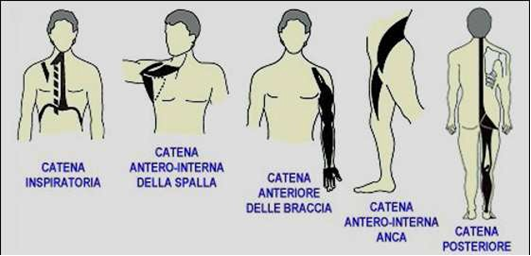
\includegraphics[width=0.7\textwidth]{027/image1.png}
\end{figure}

Il loro funzionamento, quando irrigidite, prevede che all'allungamento
di un gruppo muscolare corrisponda l'accorciamento di un altro punto
qualunque della stessa catena.

Nel corpo sono presenti diverse catene muscolari:
\begin{itemize}
\item 
 la grande sequenza del controllo anteriore: formata dal sistema
sospensore del diaframma e dei visceri, dallo sternocleidomastoideo, dal
muscolo lungo del collo, dagli scaleni, dai pilastri del diaframma,
dall'ileo-psoas, dalla fascia iliaca, dagli adduttori del pube e dal
tibiale anteriore.
\item 
la catena inspiratoria: comprende diaframma, sternocleidomastoideo,
scaleni, intercostali, spinali dorsali e piccolo pettorale
\item 
catena anterointerna della spalla: muscoli coraco-brachiale,
sottoscapolare, fascio superiore del grande pettorale
\item 
catena anteriore del braccio: coraco-brachiale, bicipite, brachiale
anteriore, lungo supinatore, muscoli anteriori dell'avambraccio,
eminenze tenar ed ipotenar
\item 
 catena antero-interna dell'anca: ileo-psoas, fascia iliaca, adduttori
del pube
\item 
catena laterale dell'anca: piramidale, grande gluteo superficiale,
tensore della fascia lata.
\end{itemize}
La RPG si basa sul principio neurofisiologico per cui ogni stimolo
nocivo provoca un aumento del tono muscolare (stato di minima tensione
dei muscoli striati in stato di riposo).

Gli organi preposti al mantenimento del tono sono i fusi neuromuscolari;
le lesioni aumentano l'attività del fuso, soprattutto per quanto
riguarda i muscoli della statica accentuazione delle risposte dei
motoneuroni $alpha$. I muscoli antigravitari subiscono modifiche a livello
dell'attività contrattile per aumento delle tensioni neuromuscolari.

 
\subsection{PROGRAMMA E PROGETTO RIABILITATIVO}


\paragraph{Obiettivi}

 

Appare un metodo valido per la riabilitazione delle malattie reumatiche:
è noto che queste malattie hanno carattere degenerativo, sistemico,
progressivo ed irreversibile; presentano, oltre ai danni indotti dalle
varie patologie, deformazioni fonte di sintomatologie dolorose le quali,
a loro volta, inducono altre deformazioni come risposte antalgiche
adattative.

\paragraph{Vantaggi della riabilitazione:}
 
 

\begin{itemize}
\item
  intervento sui distretti direttamente interessati dalla risposta
  antalgica, ristabilendo i corretti parametri muscolo-scheletrici e
  creando condizioni preventive fisiche per evitare il riproporsi del
  problema
\item
  intervento sui distretti interessati dalla patologia per recuperare
  gli assi articolari fisiologici e prevenire l'ulteriore deterioramento
  dell'articolazione.
\item 
intervento di rieducazione del paziente che gli consente di fissare
la postura globale, sia a livello corporeo che cognitivo.
\end{itemize}
 
\paragraph{Valutazione}


Prevede 4 momenti:

\begin{itemize}
\item
  Anamnesi ed acquisizione dei referti clinici e diagnostici
\item
  Analisi dello stato funzionale con valutazione della struttura
  muscolo-scheletrica, dolore, scarso equilibrio e coordinazione,
  analisi gestuale
\item
  Analisi posturale con valutazione degli assi corporei nei piani
  frontale, sagittale, trasversale, in posizione sia flessa che estesa,
  in carico e scarico
\item
  Valutazione del range di movimento
\end{itemize}

 
\section{ERGOTERAPIA o terapia occupazionale}



L'ergoterapia é una disciplina che si basa su principi della medicina e
delle scienze sociali ed é uno strumento terapeutico che deve essere
prescritto dal medico.

Si applica per persone di tutte le età che presentano disturbi delle
funzioni motoriche o delle percezioni senso-motorie, disturbi
neuropsicologici oppure disturbi di tipo psico-sociale.

Ha l'obiettivo di aiutare le persone a riacquistare nella vita
quotidiana \textbf{le capacità di azione} andate perdute o non ancora
disponibili a causa di malattie, lesioni oppure handicap. Essere capaci
di agire nella vita quotidiana significa essere in grado svolgere in
modo soddisfacente sia i compiti che ci si pone autonomamente, che
quelli che vengono posti dalla vita e dalla società.

Per poter essere capaci di agire in modo efficiente é assolutamente
necessario che le funzioni corporee, mentali e psichiche siano
sufficientemente intatte e che la persona sia in grado di interagire in
modo sensato con l'ambiente circostante. Lo \textbf{scopo principale}
dell'ergoterapia non é dunque quello di ripristinare in modo meccanico
le funzioni corporee, mentali e psichiche, ma é invece quello di fare in
modo che la persona possa nuovamente svolgere nel miglior modo possibile
i diversi ruoli della sua vita e possa quindi far fronte ai compiti ad
essa collegati.

L'ergoterapia non si occupa in primo luogo dei singoli sintomi delle
malattie, ma \textbf{della limitazione della capacità di agire.} La
disciplina si interessa di ciò che la persona non può più fare a causa
della sua malattia o della sua lesione e cerca di individuare un modo
per aiutarla.

Dopo la realizzazione di un reperto medico ergoterapeutico
differenziato, gli obiettivi individuali da raggiungere vengono
determinati insieme al paziente e/o ai suoi parenti. In seguito viene
realizzato il programma della terapia e vengono selezionati i metodi e
gli strumenti terapeutici corrispondenti.

Nel corso dei processi, gli obiettivi, i programmi terapeutici ed i
metodi di cura devono essere continuamente adattati in base alle
capacità del paziente ed alle modifiche della situazione. Nell'ambito
della terapia può anche essere necessario mettere a disposizione mezzi
ausiliari e stecche.

 
\paragraph{Ortopedia}

 

In questo settore specialistico l'ergoterapia viene utilizza la per
curare pazienti di tutte le categorie di età, che presentano disturbi di
tipo ortopedico, traumatologico o reumatologico. Tali disturbi sono, per
esempio, le malformazioni congenite del tronco, delle braccia e delle
mani, il logorio e le patologie della colonna vertebrale e di altre
articolazioni principali, le patologie infiammatorie e degenerative
delle articolazioni di origine reumatica, le lesioni alle ossa, ai
muscoli, ai tendini e ai nervi, le amputazioni, le paralisi nervose
(soprattutto nel settore delle braccia e del tronco) ed i tumori delle
ossa, dei muscoli oppure dei nervi.

La \textbf{mobilità} deve essere ripristinata, la \textbf{muscolatura}
deve essere rafforzata ed é necessario normalizzare la

 
\textbf{funzionalità e la coordinazione} delle mani e di tutte le
singole dita.
 

Nell'ambito dell'ergoterapia il paziente deve imparare ad utilizzare le
proprie forze ed a compensare gli handicap permanenti tramite la
modificazione del suo comportamento e delle sue procedure di lavoro. Ciò
può anche avvenire per mezzo del training con mezzi ausiliari speciali
(stecche realizzate dall'ergoterapeuta oppure protesi).

Le cure ergoterapeutiche in questo settore specifico comprendono per
esempio:

\begin{itemize}
\item
  Gli esercizi per migliorare la mobilità, la forza muscolare, la
  resistenza, la capacità di sopportazione e la sensibilità
\item
  Il training riferito alle attività quotidiane, per quanto riguarda
  l'autonomia personale e nella vita domestica e professionale
\item
  La consulenza ed il training per la protezione delle articolazioni
\item
  L'irrobustimento delle superfici di amputazione ed il training con le
  protesi
\item
  La realizzazione di stecche speciali per le braccia e per le mani
\end{itemize}

Le cure ergoterapeutiche attenuano le conseguenze delle patologie
fondamentali e provvedono a rafforzare e le capacità ancora disponibili.
L'obiettivo principale é quello di garantire il livello massimo
possibile di qualità della vita e di raggiungere il massimo grado
possibile di autonomia in tutti i settori della vita personale,
domestica e professionale

\section{IDROKINESITERAPIA}
 

 

Questa è una terapia che sfrutta le proprietà dell'acqua, dove si
possono fare movimenti altrimenti impossibili da effettuare a secco. Es:
un paziente con un trauma del femore non ha garanzie di recupero
nell'immediato post-operatorio, dunque si può pensare di riabilitarlo in
scarico in acqua per poi proseguire con la terapia a secco

 
\paragraph{Proprietà dell'acqua:}

 

\begin{itemize}
\item
  Il peso specifico dell'acqua è superiore a quello del corpo, e ciò
  crea la spinta di Archimede che consente il \textbf{galleggiamento};
  in queste circostanze l'escursione dell'articolazione aumenta.
\item
  Inoltre, l'acqua offre una certa resistenza e incrementa la
  \textbf{potenza muscolare}.
\item
  Infine, in acqua si stimolano \textbf{altri apparati}, primo tra tutti
  l'apparato cardiovascolare.
\end{itemize}

Il punto chiave è \textbf{l'attivazione del sistema propriocettivo} da
parte dell'acqua: la contrazione muscolare riflessa si opporrà alla
situazione di instabilità creata dall'immersione. Peraltro i
galleggianti sono in grado di perturbare ulteriormente l'equilibrio e
consentono una forte attivazione di questo sistema.

La viscosità legata all'attrito oppone una \textbf{resistenza} al
movimento, e ciò consente di sviluppare un'importante contrazione
muscolare, per un effetto di ostacolo (ex piscine col nuoto
controcorrente). In più questa resistenza può essere variata tramite
mezzi che aumentano l'attrito, ad esempio utilizzando un galleggiante di
ampia superficie (tavoletta,pull-boy).

Il \textbf{livello di immersione} ovviamente modifica il carico
sull'articolazione; ad esempio, l'immersione a livello del collo riduce
il peso al 20\%. Il livello più utilizzato è quello al bacino, 50\% del
peso, e al torace 40\%. In alcune situazioni si usa un'immersione a
livello del ginocchio per aumentare la resistenza muscolare della gamba
e della coscia (il prof consiglia di vedere sui libri la formula della
resistenza opposta dall'acqua).

 
\textbf{NB: Ricordare che il trattamento in acqua deve sempre essere
associato ad una terapia a secco, DA SOLO NON BASTA.}

\textbf{\emph{In una piscina riabilitativa l'acqua è sempre calda, con
una T attorno ai 32 gradi; al di sopra si parla} \emph{di piscina
termale.}}
 

\paragraph{EFFETTI DELL'ACQUA CALDA}: aumento della temperatura,
vasodilatazione, aumento del ritmo metabolico e respiratorio, ipotonia,
sudorazione. Per questi motivi, ovviamente non tutti i pazienti potranno
essere messi in acqua.

 
\emph{In sintesi gli effetti benefici della idrokinesiterapia sono:}
 

\begin{itemize}
\item
  \emph{Effetto antalgico, decontratturante e miorilassante, modesta
  vasodilatazione periferica con miglioramento conseguente del trofismo
  tissutale}
\item
  \emph{Effetto antinfiammatorio}
\item
  \emph{Migliora la circolazione anche sul versante venoso e
  l'escursione articolare}
\item
  \emph{Effetto sulla cute}
\item
  \emph{Effetto psicologico(il paziente è più motivato perché si vede
  eseguire un movimento altrimenti impraticabile).}
\end{itemize}

\subsection{PROGRAMMA E PROGETTO RIABILITATIVO}

\paragraph{Obiettivi}


\begin{itemize}
\item 
intervenire localmente sulla mobilizzazione delle singole
articolazioni con un miglioramento dell'escursione articolare per
esempio dopo un periodo di immobilità, nel periodo postchirurgico, dopo
una fase acuta di malattia o come preparazione preoperatoria, grazie
alla spinta di galleggiamento si riduce il peso corporeo e si facilita
il movimento che avviene in modo graduale, lento e preciso;
\item 
 potenziare la muscolatura
\item 
migliorare il controllo dell'equilibrio e del movimento
\item 
 predisporre le giuste condizioni muscolo-scheletriche all'applicazione
di altri approcci terapeutici e quindi rendere più rapidi i tempi di
recupero

 \end{itemize}
 
\subsection{CONTROINDICAZIONI PER LA TERAPIA:}

 \begin{itemize}

\item 
\textbf{assolute:} infezioni in genere, fistole, escare, micosi,
infezioni orl, infezioni urinarie, piaghe infette, congiuntiviti;
patologie cardiovascolari e respiratorie gravi come ipertensione e
ipotensione arteriosa, insufficienza respiratoria e cardiovascolare,
coronaropatie instabili, ulcere varicose.
\item 
\textbf{relative:} neoplasie, allergia a componenti dell'acqua della
piscina, mestruazioni.
 \end{itemize}
 
L'acqua stimola il senso cinestesico, ossia la capacità di riconoscere
la propria posizione nello spazio. Perciò la terapia con l'acqua può
riguardare pazienti con emiplegie, paraplegie, tetraplegia incompleta,
postumi di traumi cranici, miopatie, sclerosi multipla, morbo di
Parkinson.

La scuola francese consiglia di fare la riabilitazione della spalla già
nel postoperatorio in completa immersione in acqua, usando cerotti
impermeabili, perché qui non c'è alcuna resistenza.

In ambito traumatologico, l'idrokinesiterapia è consigliata in caso di
paramorfismi e dismorfismi, postumi di fratture ossee e legamentose,
postumi di protesizzazioni, distrazioni, strappi muscolari, processi
degenerativi articolari (artrosici).

